\documentclass{article}
\usepackage[utf8]{inputenc}
\usepackage{amsmath}
\usepackage[a4paper,body={140mm,250mm}]{geometry}

\usepackage{graphicx} 
\usepackage{array} 
%\usepackage{newtxtext,newtxmath}
%\usepackage[varl]{inconsolata}

\begin{document}
\begin{titlepage}
  \begin{flushleft}\scshape
    Lund University\\
    Automatic Control\\[\smallskipamount]
    FRTN70 Project in Systems, Control and Learning\\
    Spring 2021
  \end{flushleft}
  \vspace*{0pt plus 0.3fill}
  \begin{center}
    \huge \textbf{Reinforcement Learning for Double Pendulum}\\[4mm]     
    \large\textbf{Project Plan Group H}\\[5mm]
         Cem Alpturk\footnote{\texttt{ce5368al-s@student.lu.se}}\quad
         Pukashawar Pannu\footnote{\texttt{pu6218pa-s@student.lu.se}}
  \end{center}
\begin{center}
    Project Advisor: Emil Vladu
\end{center}
\vfill
\end{titlepage}        

\section{Project Purpose}
The goal of this project is to teach a model to control a double pendulum on a cart to be standing upright, in it's equilibrium point, using reinforcement learning.

\section{Equipments and Material} \label{sec:equipment}
This project does not require any physical equipment.
It will be fully simulated.

\section{Modelling and System Design}
Focus of the project is to train a controller for the dobule pendulum and not to model the actual double pendulum on a cart.


\section{Division of Labour} \label{sec:division}
We have decided to split our project into three parts: Setting up Environment, Train the Agents, Presentation. 

\subsection{Setting up Environment}
In order to teach an agent to control a double pendulum we need to simulate it.
This section is about setting up the requirements for the training phase.
Equations for the double pendulum on a cart will be researched online and from other available sources and implemented using Python.
Model will be verified by comparing with online models and an attempt will be made to animate the results to see if it looks as expected.

\subsection{Training the Agents}
This will be the main focus of the project, which is to create models and train them to control the double pendulum.
The training will utilize reinforcement learning where the agent will learn from experience by trial and error.
If the agent manages to keep the pendulum upright for a long enough time, the time has not been decided as of yet, it is considered to have solved the problem.
\subsubsection{Deciding Network Architecture}
Before we start training the models we need to decide on what type of architecture to use. We need to investigate the advantages and disadvantages of different types of networks such as feed forward, recurrent networks etc.
\subsubsection{Deciding Simulation Conditions}
We need to define a reward system for the training process, together with a completion and a failure condition.

\subsection{Demo and Report}
Create a basic demo showing our results and write a detailed report.

\section{Time Plan}
\subsection{Subtasks}
	\begin{itemize}
		\item Search online sources for the equations of motion for the double pendulum and implement it in Python. Compare pendulum behavior to other available simulations in order to make sure that the behavior is accurate. \textbf{Estimated Deadline}: \textbf{Apr 5}
		\item Animate the model using available Python libraries. \textbf{Estimated Deadline}: \textbf{Apr 5}
		\item Set up Gym Environment and documentation. \textbf{Estimated Deadline}: \textbf{Apr 9}
		\item Practice Reinforcement Learning on a more basic problem. \textbf{Estimated Deadline}: \textbf{Apr 9}
		\item Decide on the network architecture for the model. \textbf{Estimated Deadline}: \textbf{Apr 16}
		\item Decide on a reward system for the model. \textbf{Estimated Deadline}: \textbf{Apr 21}
		\item Decide on a completion condition. \textbf{Estimated Deadline}: \textbf{Apr 16}
		\item Decide on a fail condition. \textbf{Estimated Deadline}: \textbf{Apr 16}
		\item Train a model that is able to keep both pendulum in upright position without any disturbances. \textbf{Estimated Deadline}: \textbf{Apr 23}
		\item Train a model that is able to keep both pendulums in upright position in the presence of disturbances. \textbf{Estimated Deadline}: \textbf{Apr 27}
		\item Finalize documentation. \textbf{Estimated Deadline}: \textbf{May 5}
		\item If there is enough time, train different models to balance the pendulums in the other equilibrium points. 
		\item If there is enough time, train a model that can utilize swing-up and stay in balance. 
		\item If there is enough time, write a demo in Jupyter Notebook so that other students can run it easily. 
	\end{itemize}
    
\subsection{Important dates}
    \begin{itemize}
        \item Mar 29 -  Hand in project plan.
        \item Apr 22 - Feedback seminar 1 on the modeling and design.
        \item May 5 - Report should be pushed to git to allow peer review by other groups.
        \item May 11 - Peer review done
        \item May 12 - Feedback seminar 2 on the design and implementation.
        \item May 20 - Project done and demonstrated and final report handed in
        \item May 27 - Demo film upload and peer review of final report done
        \item June 3 - Final presentation and demonstration and revised final report handed in
    \end{itemize}
    
    \subsection{Gantt Chart}
    The project plan can be seen in estimated duration in days, plotted in Figure~\ref{fig:gantt}
    \begin{figure}
    		\centering
    		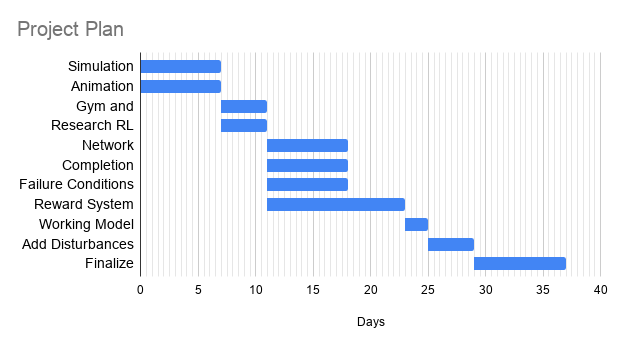
\includegraphics[width=0.95\textwidth]{figures/Project_plan.png}
    		\caption{The Gantt chart showing the work flow.} \label{fig:gantt}
    \end{figure}

%\subsection{Gantt Chart}
%    We have formalized the time plan as a Gantt chart. The major tasks can be seen plotted in Figure~\ref{fig:gantt}.
%    \begin{figure}
%        \centering
%        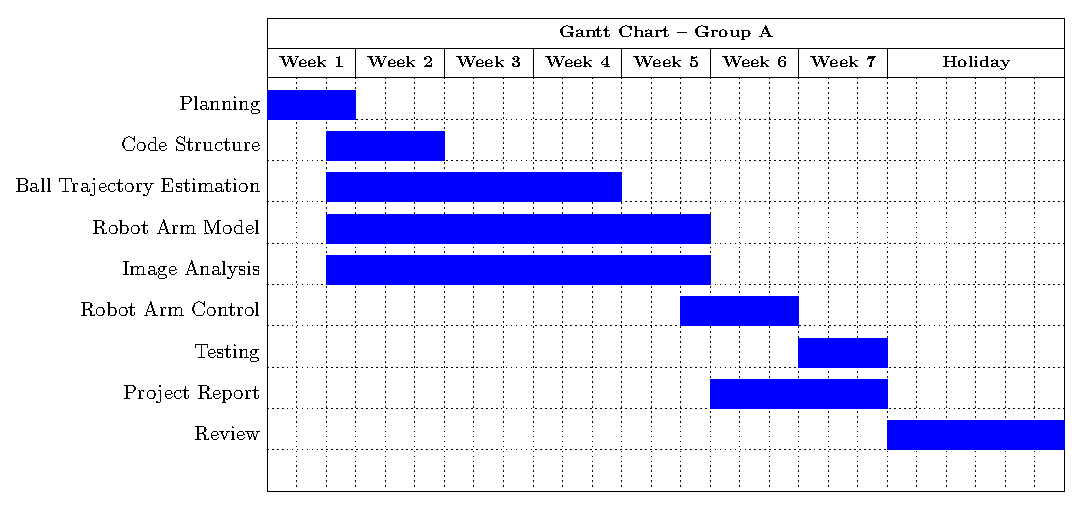
\includegraphics[width=0.95\textwidth]{figures/gantt}
%        \caption{The Gantt chart describing the work flow of our project.}
%        \label{fig:gantt}
%    \end{figure}

\end{document}
